\chapter{Appendix}

\section{Static Obstacle Collision checking}
\label{static_obst_appendix}
Static obstacle checking described in section \ref{osbtacle_check_satic} works on the concept that it is sufficient to check the lateral distance (D) between the obstacle and the ego at minimum and maximum of ego D (lateral coordinate) in the longitudinal intersection region.

Let $f(x)$ be a function of lateral motion D in intersection interval $[a,b]$, $f(x)\ge f(c)$ (respectively, $f(x)\le f(c)$), then $f(c)$ is the absolute minimum (respectively, absolute ) local maximum value of $f(x)$ on $[a,b]$ and vice versa. 

If $f(x)$ is continuous on $[a, b]$ and differentiable in $(a, b)$, a point $c$ in $[a, b]$ is a critical point of $f(x)$ if either $f'(c) =0$ or $f'(c)$ does not exist. The 

If $f(x)$ is continuous on $[a,b]$ and differentiable in (a,b), and if for some $c$ in $(a,b)$, if $f(c)$ is local minima or maxima then $c$ must be a critical point. Any absolute maximum or minimum will take place at boundaries or critical points inside the interval $(a,b)$. 


\begin{figure}
	\centering
	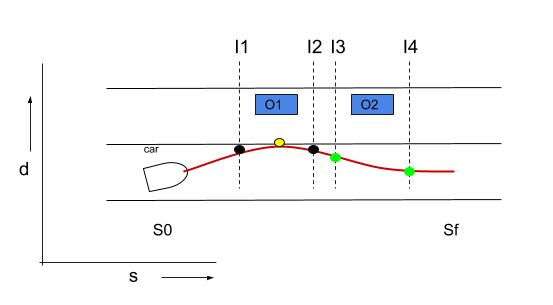
\includegraphics[width=0.8\textwidth]{Images/appendix/staticpoints.jpg}
	\caption{Static Obstacle Collision check - Lateral distance between obstacle O1 and trajectory is checked at points with black dots, distance at green dots is checked for obstacle O2.}
	\label{cstat_coll_appen}
\end{figure}

Consider $f(x) = x^3 - x^2 -x + 12$ with intersection interval in $[0,2]$, critical points are at $x=-1/3$ which is not in intersection and $x=1$ is in the intersection interval. Thus it is sufficient to check for values of $f(x)$ at [0,1,2] to find minima and maxima. 

In the figure \ref{cstat_coll_appen}, for obstacle O1 it is necessary to check collision at critical point that lies in [I1,I2] represented with yellow dot and at the borders represented with black dots. For the second obstacle O2 it is sufficient to check at the borders of interval [I3,I4]. If the critical points and the borders have sufficient lateral distance to the obstacle then the rest of the points on trajectory will also have safe lateral distance and it is not needed to check for collision at other points. 

%Proof thats its sufficient to check only at borders and only if global min or max exists in the intersection interval for collision checking with static obstacles
%https://www.math.wvu.edu/~hjlai/Words2Algebra/MinMax_Closed_Interva.pdf

\section{Dynamic Obstacle Collision checking}
\label{dynamic_obst_appendix}

In the proposed algorithm in section \ref{obstacle_check_dynamic}, for collision checking with respect to dynamic obstacles time difference only at the borders where lateral and longitudinal coordinates intersect is checked. This is a valid assumption when the vehicle velocity is linear but the trajectory will end in collision if a minimum buffer time is not maintained. 

\begin{figure}
	\centering
	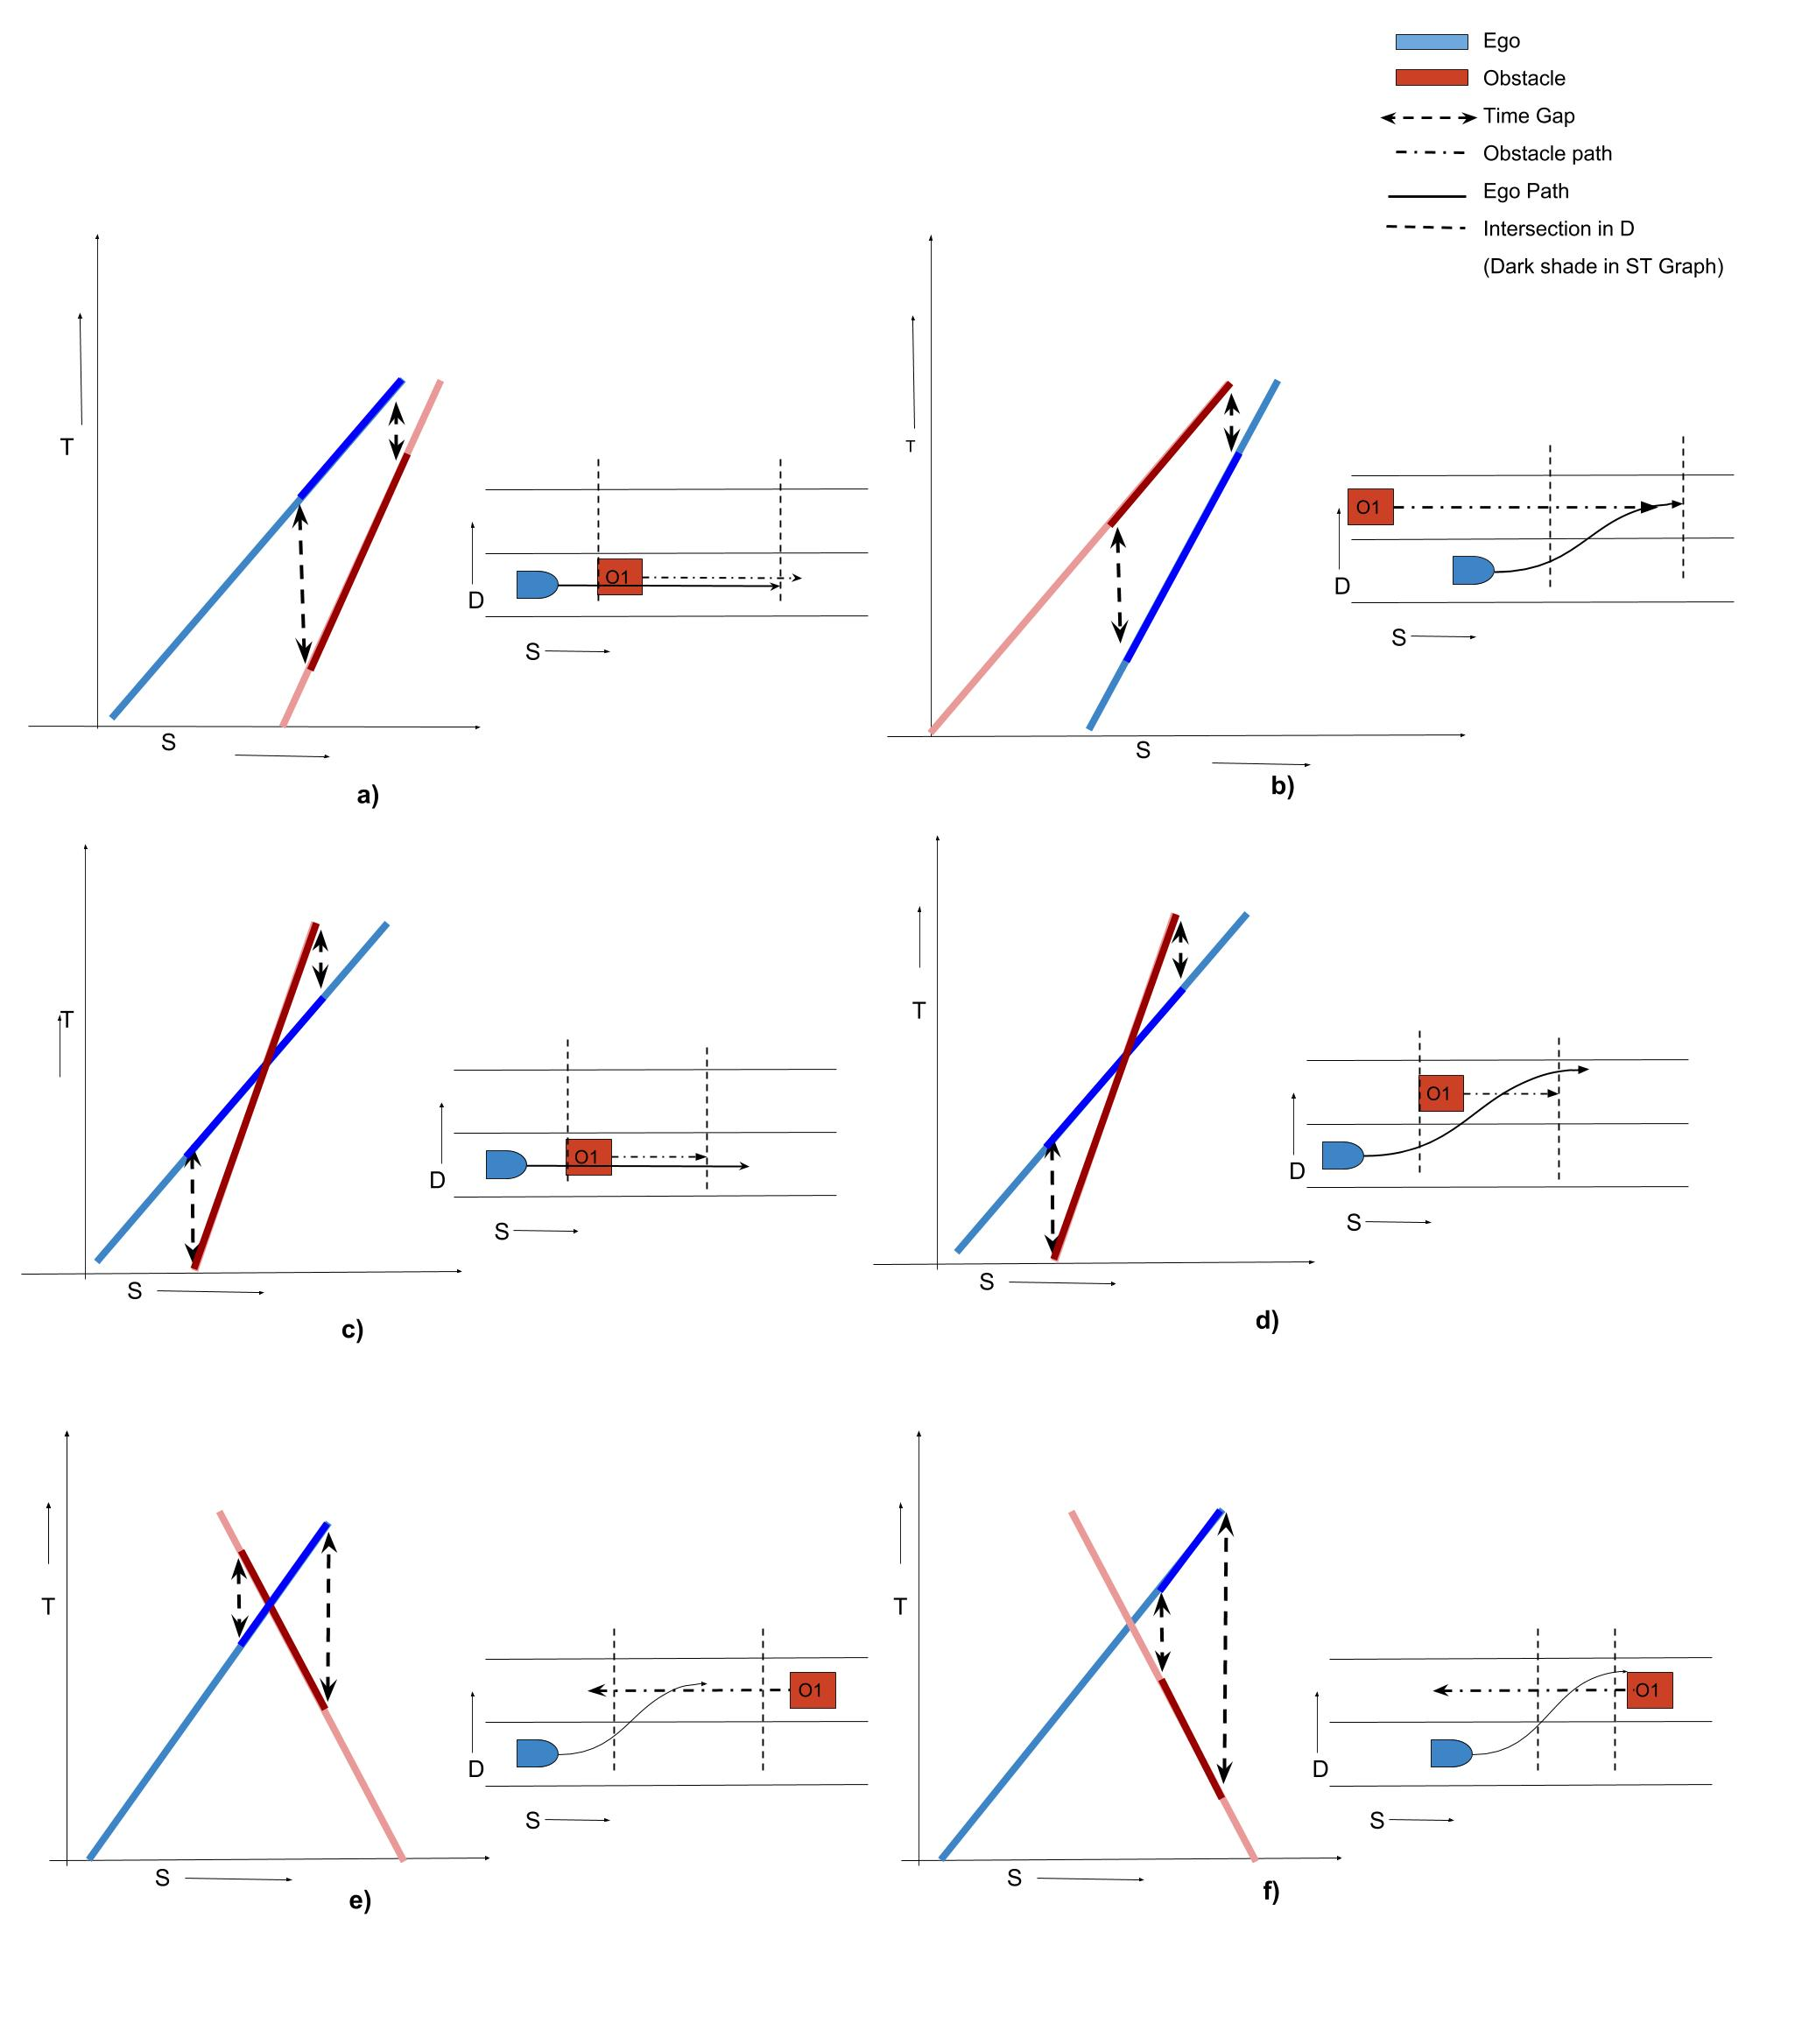
\includegraphics[width=1.1\textwidth]{Images/appendix/dynamic_collision_lines.jpg}
	\caption{ddd.}
	\label{dynamic_appendix}
\end{figure}




Proof that the approximating collision checking for dynamic obstacles as straight line is fine. 

